\documentclass[tikz,14pt,fleqn]{article}


\usepackage[utf8]{inputenc}
\usepackage[margin=1in]{geometry}
\usepackage[titletoc,title]{appendix}
\usepackage{latexsym}
\usepackage{amssymb}
\usepackage{gensymb}
\usepackage{amsmath}
\usepackage{amsfonts}
\usepackage[dvipsnames]{xcolor}
\usepackage{multicol}
\usepackage{graphicx}
\usepackage{fancyhdr}
\usepackage[linguistics]{forest}
\usepackage{colortbl}
\usepackage{pdfpages}
\usepackage{wrapfig}
\usepackage{cleveref}


% to fixme
\usepackage{xcolor} 
\definecolor{FIXMECOLOR}{rgb}{1,0,0}
\newcommand{\FIXME}[1]{{\color{FIXMECOLOR}{\textbf{FIXME: #1}}}} 

%% For plotting
\usepackage{pgfplots}
\pgfplotsset{width=10cm,compat=1.9}
\usepgfplotslibrary{external}
\tikzexternalize
%%
\usepackage{dirtree}
\usepackage{subcaption}
\usepackage{xifthen}% provides \isempty test
\usepackage{glossaries}

\captionsetup[subfigure]{labelformat=empty}
\definecolor{color1}{HTML}{0B0C10}
\definecolor{color2}{HTML}{1F2833}
\definecolor{color3}{HTML}{C5C6C7}
\definecolor{color4}{HTML}{66FCF1}
\definecolor{color5}{HTML}{45A29E}

\pagestyle{fancy}
\fancyhf{}
%%%%%%%%%%%%%%%%%%%%%%%%%%%%
%% VARIABLES
\newcommand\namesurname{Albert Cerfeda\\Alessandro Gobbetti}
\newcommand\assignment{Assignment 2}

\newcommand\subject{Computer Graphics}
\newcommand\documentdate{3.10.2022}

% Title content
%%%%%%%%%%%%%%%%%%%%%%%%%%%%
\rhead{\assignment}
\lhead{\namesurname}
%%%%%%%%%%%%%%%%%%%%%%%%%%%%
\rfoot{Page \thepage}
\setlength{\parindent}{0pt}

\newcommand\xdownarrow[1][2ex]{%
   \mathrel{\rotatebox{90}{$\xleftarrow{\rule{#1}{0pt}}$}}
}

\begin{document}

\begin{titlepage}
   \begin{center}
       \vspace*{1cm}

       \textbf{\Large{Homework Assignment}}

       \vspace{0.5cm}
        \textbf{\subject}\\[5mm]
       \assignment
        
            
       \vspace{1.8cm}

        \namesurname
       \tableofcontents

       \vspace*{\fill}
     
       
\includegraphics[width=0.4\textwidth]{fig/logo.png}
       
        \documentdate \\
        Università della Svizzera italiana\\
        Faculty of Informatics\\
        Switzerland\\

   \end{center}
\end{titlepage}


%%%%%%%%%%%%%%%%%%%%%%%%%%%%%%%%%%%%%%%%%%%%%%%%%%%%
%%%%%%  CONTENT START   %%%%%%%%%%%%%%%%%%%%%%%%%%%%
% color	white, black, red, green, blue, cyan, magenta, yellow
% thickness	ultra thin, very thin, thin, thick, very thick, ultra thick
% dots (/loosely/densely) + dotted, dashed, dashdotted
\section{Exercise 2}

The vector towards the directional light source: $ l = \begin{pmatrix} 1 \\ 2 \\ 2 \end{pmatrix}$.

The position of the camera: $c = \begin{pmatrix} 4 \\ 6 \\ 7 \end{pmatrix}$.

Given a plain $y = 0$ we have the normal $ n = (0, 1, 0)^T $

\subsection{Task 1}

We know that the reflected ray $r$ is:
\begin{align*}
   r 
   &= 2n \cdot \langle n, l \rangle - l \\
   &= 2\begin{pmatrix} 0 \\ 1 \\ 0 \end{pmatrix} \cdot \langle \begin{pmatrix} 0 \\ 1 \\ 0 \end{pmatrix}, \begin{pmatrix} 1 \\ 2 \\ 2 \end{pmatrix} \rangle - \begin{pmatrix} 1 \\ 2 \\ 2 \end{pmatrix}\\
   &= 2\begin{pmatrix} 0 \\ 1 \\ 0 \end{pmatrix} \cdot 2 - \begin{pmatrix} 1 \\ 2 \\ 2 \end{pmatrix}\\
   &= \begin{pmatrix} 0 \\ 4 \\ 0 \end{pmatrix} - \begin{pmatrix} 1 \\ 2 \\ 2 \end{pmatrix}\\
   &= \begin{pmatrix} -1 \\ +2 \\ -2 \end{pmatrix}
\end{align*}



So: $ c - \beta r = p $
\[
   \begin{pmatrix} 4 \\ 6 \\ 7 \end{pmatrix} - \beta \begin{pmatrix} -1 \\ +2 \\ -2 \end{pmatrix} = \begin{pmatrix} x \\ y \\ z \end{pmatrix}
\]
Since $y$ is on the plain $y = 0$ we have $y = 0$ and we can solve the system:
\[
   \begin{cases}
      4 - \beta (-1) = x \\
      6 - \beta (2) = 0 \\
      7 - \beta (-2) = z
   \end{cases}
\]
\[
   \begin{cases}
      4 + \beta = x \\
      6 - 2\beta = 0 \\
      7 + 2\beta = z
   \end{cases}
\]
\[
   \begin{cases}
      4 + \beta = x \\
      \beta = 3 \\
      7 + 2\beta = z
   \end{cases}
\]
\[
   \begin{cases}
      x = 4+3=7 \\
      \beta = 3 \\
      z = 7 + 2 \cdot 3 = 13
   \end{cases}
\]
So the intersection point is: $p = \begin{pmatrix} 7 \\ 0 \\ 13 \end{pmatrix}$


\subsection{Task 2}



\newpage
\section{Exercise 3}


\begin{wrapfigure}{r}{0.3\textwidth}
   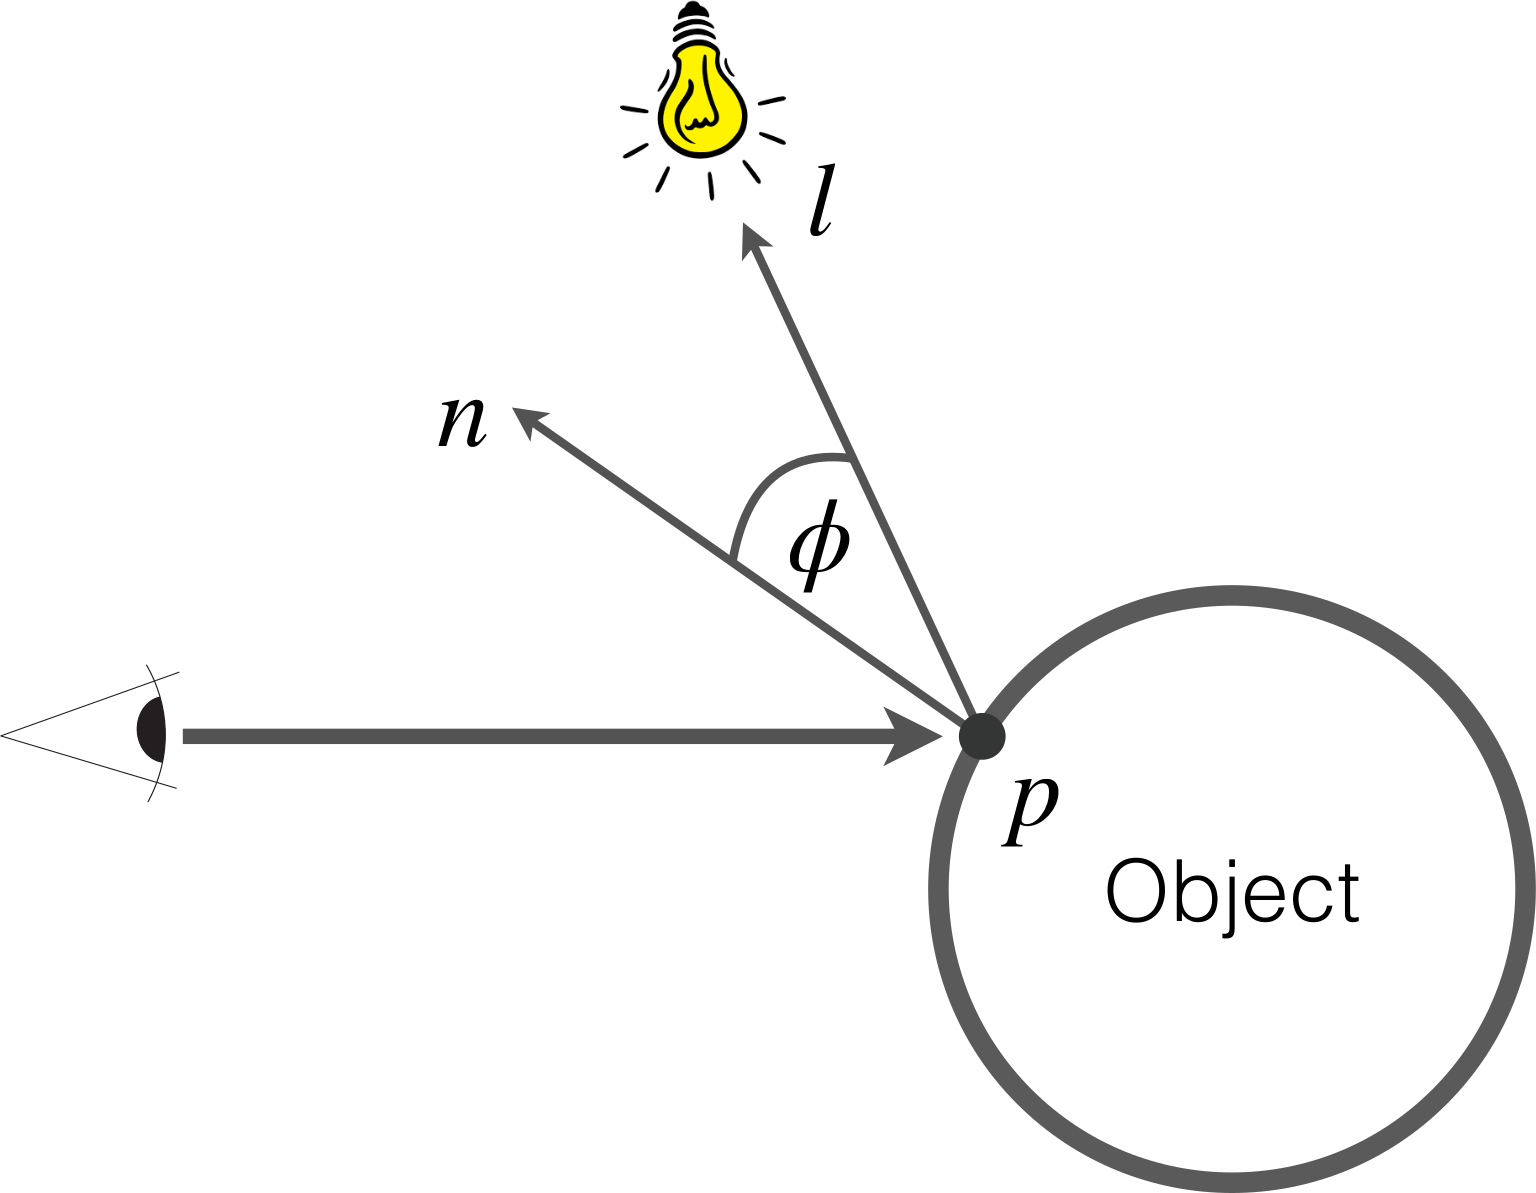
\includegraphics[width=0.9\linewidth]{fig/Lambert_cosine_law.png} 
   \caption{Lambert's cosine law}
   \label{fig:lambert}
\end{wrapfigure}


The Phong lighting model is an empirical model to describe the illumination of the points representing an object.
According to this model, the color of every pixel is modulated by the cosine of the angle between the normal vector and 
the light direction (Lambert's cosine law) as shown in \cref{fig:lambert}.


But we notice that some objects does not follow the Phong illumination model and apper flat. An example is the full moon: 
ignoring the shading artifacts caused by craters, it appears as a white disk with constant brightness
rather than a sphere shaded according to the Phong illumination.

This effect is due to the roughness of the surface. 
When rays hit the surface, they are reflected in random directions, including the direction of the camera.
As shown in \cref{fig:increasing_roughness}, increasing the surface roughness makes the object appear flatter. 

\begin{figure}[!hb]
   \centering
   \begin{minipage}{.5\textwidth}
     \centering
     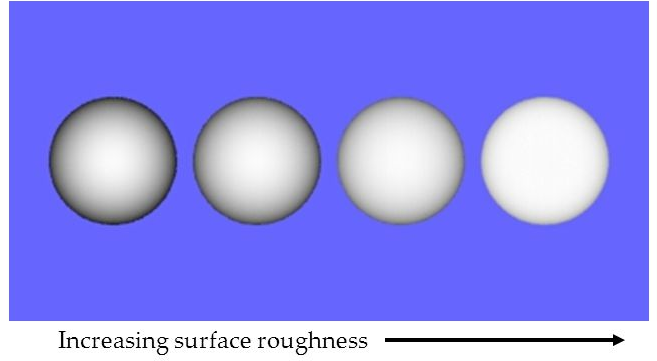
\includegraphics[width=.8\linewidth]{fig/increasing_surface_roughness.png}
     \captionof{figure}{A figure}
     \label{fig:increasing_roughness}
   \end{minipage}%
   \begin{minipage}{.5\textwidth}
     \centering
     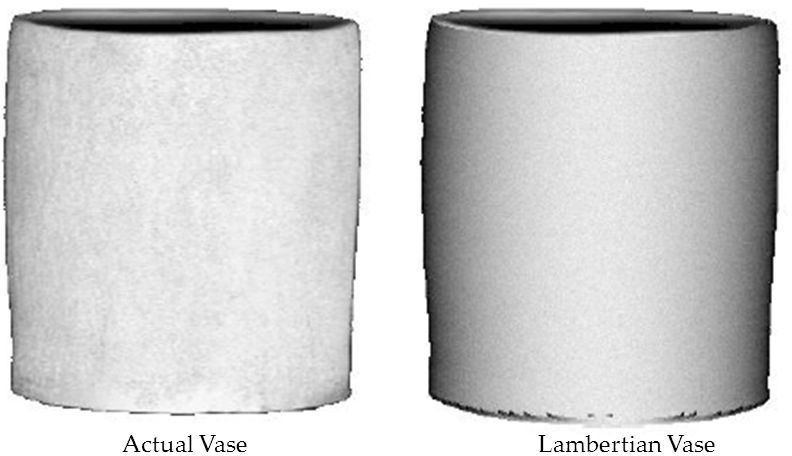
\includegraphics[width=.8\linewidth]{fig/actual_VS_lambertian-vase.png}
     \captionof{figure}{Another figure}
     \label{fig:vases}
   \end{minipage}
\end{figure}

In \cref{fig:vases} we note that the lambertian model doesn't work correctly with rough materials.

To render rough objects more accurately, the Oren-Nayar model is often used, which takes into account surface roughness (\cref{fig:Oren-Nayar}).

When the roughness is set to 0 the Oren-Nayar model simplifies to the Lambertian model.


\begin{figure}[!h]
   \centering
   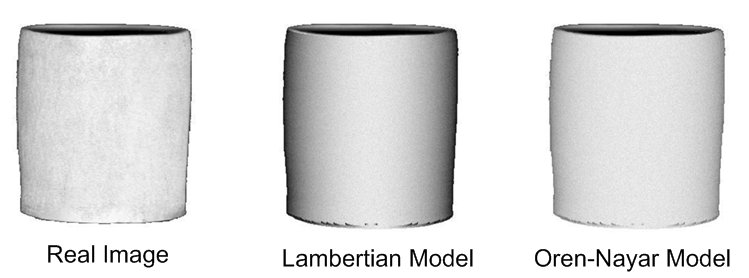
\includegraphics[width=0.7\linewidth]{fig/Oren-Nayar-Model-Vase.png} 
   \caption{Oren-Nayar model}
   \label{fig:Oren-Nayar}
\end{figure}




% \FIXME{fix this}

% The Phong lighting model is used for \textit{point light} sources.
% The light intensity levels in this case depend on the angle at which the light rays hit the surface. The smaller the angle between the ray and the surface normal, the higher resulting illumination.\\

% Even though the Sun is to be considered a \textit{point light} source,
% it is so far away that once the rays reach the moon they are almost perfectly parallel,
% behaving like a \textit{directional light} source by irradiating the moon surface equally.\\


\section{Exercise 4}

\clearpage


\end{document}

